\documentclass{book}
\usepackage[a4paper,top=2.5cm,bottom=2.5cm,left=2.5cm,right=2.5cm]{geometry}
\usepackage{makeidx}
\usepackage{natbib}
\usepackage{graphicx}
\usepackage{multicol}
\usepackage{float}
\usepackage{listings}
\usepackage{color}
\usepackage{ifthen}
\usepackage[table]{xcolor}
\usepackage{textcomp}
\usepackage{alltt}
\usepackage{ifpdf}
\ifpdf
\usepackage[pdftex,
            pagebackref=true,
            colorlinks=true,
            linkcolor=blue,
            unicode
           ]{hyperref}
\else
\usepackage[ps2pdf,
            pagebackref=true,
            colorlinks=true,
            linkcolor=blue,
            unicode
           ]{hyperref}
\usepackage{pspicture}
\fi
\usepackage[utf8]{inputenc}
\usepackage{mathptmx}
\usepackage[scaled=.90]{helvet}
\usepackage{courier}
\usepackage{sectsty}
\usepackage{amssymb}
\usepackage[titles]{tocloft}
\usepackage{doxygen}
\lstset{language=C++,inputencoding=utf8,basicstyle=\footnotesize,breaklines=true,breakatwhitespace=true,tabsize=4,numbers=left }
\makeindex
\setcounter{tocdepth}{3}
\renewcommand{\footrulewidth}{0.4pt}
\renewcommand{\familydefault}{\sfdefault}
\hfuzz=15pt
\setlength{\emergencystretch}{15pt}
\hbadness=750
\tolerance=750
\begin{document}
\hypersetup{pageanchor=false,citecolor=blue}
\begin{titlepage}
\vspace*{7cm}
\begin{center}
{\Large Gestion de Commande \\[1ex]\large 1.\-0 }\\
\vspace*{1cm}
{\large Generated by Doxygen 1.8.2}\\
\vspace*{0.5cm}
{\small Mon Oct 8 2012 12:20:14}\\
\end{center}
\end{titlepage}
\clearemptydoublepage
\pagenumbering{roman}
\tableofcontents
\clearemptydoublepage
\pagenumbering{arabic}
\hypersetup{pageanchor=true,citecolor=blue}
\chapter{Namespace Index}
\section{Packages}
Here are the packages with brief descriptions (if available)\-:\begin{DoxyCompactList}
\item\contentsline{section}{\hyperlink{namespacegestion_commande}{gestion\-Commande} }{\pageref{namespacegestion_commande}}{}
\end{DoxyCompactList}

\chapter{Hierarchical Index}
\section{Class Hierarchy}
This inheritance list is sorted roughly, but not completely, alphabetically\-:\begin{DoxyCompactList}
\item \contentsline{section}{gestion\-Commande.\-Lire}{\pageref{classgestion_commande_1_1_lire}}{}
\item \contentsline{section}{gestion\-Commande.\-main}{\pageref{classgestion_commande_1_1main}}{}
\item Serializable\begin{DoxyCompactList}
\item \contentsline{section}{gestion\-Commande.\-Article}{\pageref{classgestion_commande_1_1_article}}{}
\begin{DoxyCompactList}
\item \contentsline{section}{gestion\-Commande.\-Article\-Produit}{\pageref{classgestion_commande_1_1_article_produit}}{}
\end{DoxyCompactList}
\item \contentsline{section}{gestion\-Commande.\-Client}{\pageref{classgestion_commande_1_1_client}}{}
\item \contentsline{section}{gestion\-Commande.\-Commande}{\pageref{classgestion_commande_1_1_commande}}{}
\end{DoxyCompactList}
\end{DoxyCompactList}

\chapter{Class Index}
\section{Class List}
Here are the classes, structs, unions and interfaces with brief descriptions\-:\begin{DoxyCompactList}
\item\contentsline{section}{\hyperlink{classgestion_commande_1_1_article}{gestion\-Commande.\-Article} }{\pageref{classgestion_commande_1_1_article}}{}
\item\contentsline{section}{\hyperlink{classgestion_commande_1_1_article_produit}{gestion\-Commande.\-Article\-Produit} }{\pageref{classgestion_commande_1_1_article_produit}}{}
\item\contentsline{section}{\hyperlink{classgestion_commande_1_1_client}{gestion\-Commande.\-Client} }{\pageref{classgestion_commande_1_1_client}}{}
\item\contentsline{section}{\hyperlink{classgestion_commande_1_1_commande}{gestion\-Commande.\-Commande} }{\pageref{classgestion_commande_1_1_commande}}{}
\item\contentsline{section}{\hyperlink{classgestion_commande_1_1_lire}{gestion\-Commande.\-Lire} }{\pageref{classgestion_commande_1_1_lire}}{}
\item\contentsline{section}{\hyperlink{classgestion_commande_1_1main}{gestion\-Commande.\-main} }{\pageref{classgestion_commande_1_1main}}{}
\end{DoxyCompactList}

\chapter{File Index}
\section{File List}
Here is a list of all files with brief descriptions\-:\begin{DoxyCompactList}
\item\contentsline{section}{C\-:/\-Users/\-Rouinsard/\-Java/\-Gestion de commandes/src/gestion\-Commande/\hyperlink{_article_8java}{Article.\-java} }{\pageref{_article_8java}}{}
\item\contentsline{section}{C\-:/\-Users/\-Rouinsard/\-Java/\-Gestion de commandes/src/gestion\-Commande/\hyperlink{_article_produit_8java}{Article\-Produit.\-java} }{\pageref{_article_produit_8java}}{}
\item\contentsline{section}{C\-:/\-Users/\-Rouinsard/\-Java/\-Gestion de commandes/src/gestion\-Commande/\hyperlink{_client_8java}{Client.\-java} }{\pageref{_client_8java}}{}
\item\contentsline{section}{C\-:/\-Users/\-Rouinsard/\-Java/\-Gestion de commandes/src/gestion\-Commande/\hyperlink{_commande_8java}{Commande.\-java} }{\pageref{_commande_8java}}{}
\item\contentsline{section}{C\-:/\-Users/\-Rouinsard/\-Java/\-Gestion de commandes/src/gestion\-Commande/\hyperlink{_lire_8java}{Lire.\-java} }{\pageref{_lire_8java}}{}
\item\contentsline{section}{C\-:/\-Users/\-Rouinsard/\-Java/\-Gestion de commandes/src/gestion\-Commande/\hyperlink{main_8java}{main.\-java} }{\pageref{main_8java}}{}
\end{DoxyCompactList}

\chapter{Namespace Documentation}
\hypertarget{namespacegestion_commande}{\section{Package gestion\-Commande}
\label{namespacegestion_commande}\index{gestion\-Commande@{gestion\-Commande}}
}
\subsection*{Classes}
\begin{DoxyCompactItemize}
\item 
class \hyperlink{classgestion_commande_1_1_article}{Article}
\item 
class \hyperlink{classgestion_commande_1_1_article_produit}{Article\-Produit}
\item 
class \hyperlink{classgestion_commande_1_1_client}{Client}
\item 
class \hyperlink{classgestion_commande_1_1_commande}{Commande}
\item 
class \hyperlink{classgestion_commande_1_1_lire}{Lire}
\item 
class \hyperlink{classgestion_commande_1_1main}{main}
\end{DoxyCompactItemize}

\chapter{Class Documentation}
\hypertarget{classgestion_commande_1_1_article}{\section{gestion\-Commande.\-Article Class Reference}
\label{classgestion_commande_1_1_article}\index{gestion\-Commande.\-Article@{gestion\-Commande.\-Article}}
}
Inheritance diagram for gestion\-Commande.\-Article\-:\begin{figure}[H]
\begin{center}
\leavevmode
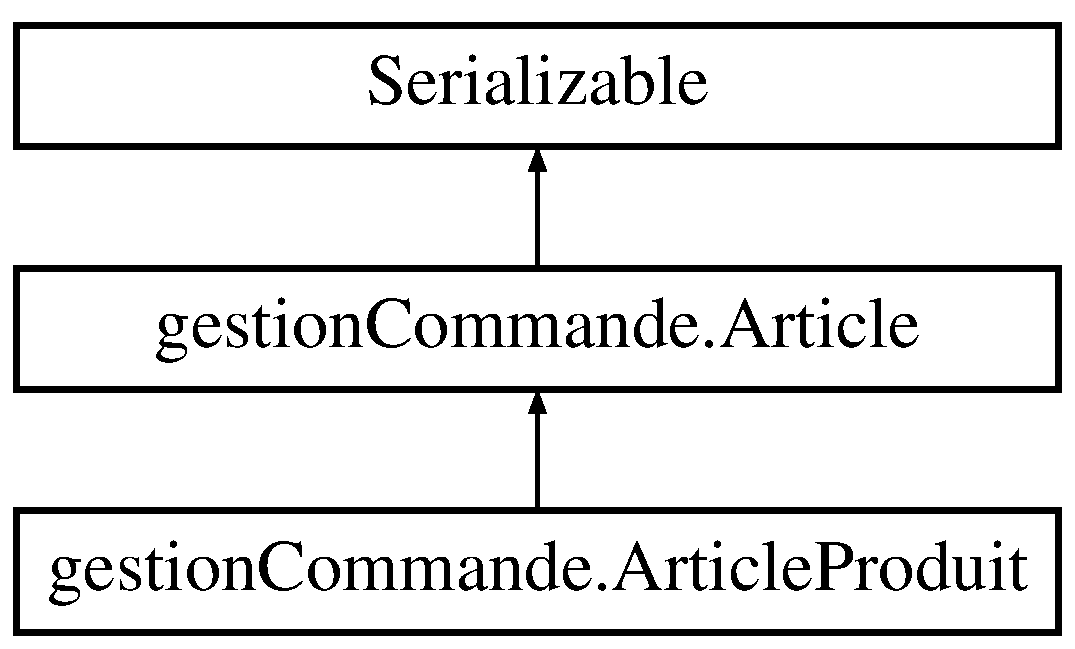
\includegraphics[height=3.000000cm]{classgestion_commande_1_1_article}
\end{center}
\end{figure}
\subsection*{Public Member Functions}
\begin{DoxyCompactItemize}
\item 
void \hyperlink{classgestion_commande_1_1_article_a9cbf8063f8e987a49d420ada8232cdfd}{saisir\-Article} ()
\begin{DoxyCompactList}\small\item\em Methode permettant la saisie d'un article. \end{DoxyCompactList}\item 
void \hyperlink{classgestion_commande_1_1_article_a3a5a28348928a6b88b337f46a88026e1}{afficher\-Article} ()
\begin{DoxyCompactList}\small\item\em Methode permettant d'afficher l'article. \end{DoxyCompactList}\item 
void \hyperlink{classgestion_commande_1_1_article_aba22b733dd82931721613a0e4338ab9f}{saisir\-Prix\-Unitaire} ()
\begin{DoxyCompactList}\small\item\em Methode permettant de saisir le prix a l'unite. \end{DoxyCompactList}\item 
String \hyperlink{classgestion_commande_1_1_article_a6206b8fb5eb14b54eefb9cd48ed50ac1}{get\-Nom\-Article} ()
\begin{DoxyCompactList}\small\item\em Methode permettant de recuperer le nom de l'article. \end{DoxyCompactList}\item 
float \hyperlink{classgestion_commande_1_1_article_a67b9ca3be955dd04c9aa3707b65b43c7}{get\-Prix\-Unitaire} ()
\begin{DoxyCompactList}\small\item\em Methode permettant de recuperer le prix unitaire de l'article. \end{DoxyCompactList}\item 
int \hyperlink{classgestion_commande_1_1_article_a45aef0c035bb11c4be39787f2c9089cd}{get\-Stock} ()
\begin{DoxyCompactList}\small\item\em Methode permettant de recuperer la quantite en stock de l'article. \end{DoxyCompactList}\end{DoxyCompactItemize}


\subsection{Detailed Description}
La classe \hyperlink{classgestion_commande_1_1_article}{Article} sert a instancier de nouveaux articles. Les articles sont renseignes par leur nom, leur prix a l'unite et leur quantite en stock. La classe \hyperlink{classgestion_commande_1_1_article}{Article} implemente l'interface Serializable. \begin{DoxyAuthor}{Author}
Rouinsard 
\end{DoxyAuthor}


Definition at line 9 of file Article.\-java.



\subsection{Member Function Documentation}
\hypertarget{classgestion_commande_1_1_article_a3a5a28348928a6b88b337f46a88026e1}{\index{gestion\-Commande\-::\-Article@{gestion\-Commande\-::\-Article}!afficher\-Article@{afficher\-Article}}
\index{afficher\-Article@{afficher\-Article}!gestionCommande::Article@{gestion\-Commande\-::\-Article}}
\subsubsection[{afficher\-Article}]{\setlength{\rightskip}{0pt plus 5cm}void gestion\-Commande.\-Article.\-afficher\-Article (
\begin{DoxyParamCaption}
{}
\end{DoxyParamCaption}
)}}\label{classgestion_commande_1_1_article_a3a5a28348928a6b88b337f46a88026e1}


Methode permettant d'afficher l'article. 

Cette methode permet d'afficher le nom, le prix a l'unite et la quantite en stock de l'article selectionne. 

Definition at line 29 of file Article.\-java.

\hypertarget{classgestion_commande_1_1_article_a6206b8fb5eb14b54eefb9cd48ed50ac1}{\index{gestion\-Commande\-::\-Article@{gestion\-Commande\-::\-Article}!get\-Nom\-Article@{get\-Nom\-Article}}
\index{get\-Nom\-Article@{get\-Nom\-Article}!gestionCommande::Article@{gestion\-Commande\-::\-Article}}
\subsubsection[{get\-Nom\-Article}]{\setlength{\rightskip}{0pt plus 5cm}String gestion\-Commande.\-Article.\-get\-Nom\-Article (
\begin{DoxyParamCaption}
{}
\end{DoxyParamCaption}
)}}\label{classgestion_commande_1_1_article_a6206b8fb5eb14b54eefb9cd48ed50ac1}


Methode permettant de recuperer le nom de l'article. 

\begin{DoxyReturn}{Returns}
this.\-nom\-Article Correspond au nom de l'article. 
\end{DoxyReturn}


Definition at line 44 of file Article.\-java.

\hypertarget{classgestion_commande_1_1_article_a67b9ca3be955dd04c9aa3707b65b43c7}{\index{gestion\-Commande\-::\-Article@{gestion\-Commande\-::\-Article}!get\-Prix\-Unitaire@{get\-Prix\-Unitaire}}
\index{get\-Prix\-Unitaire@{get\-Prix\-Unitaire}!gestionCommande::Article@{gestion\-Commande\-::\-Article}}
\subsubsection[{get\-Prix\-Unitaire}]{\setlength{\rightskip}{0pt plus 5cm}float gestion\-Commande.\-Article.\-get\-Prix\-Unitaire (
\begin{DoxyParamCaption}
{}
\end{DoxyParamCaption}
)}}\label{classgestion_commande_1_1_article_a67b9ca3be955dd04c9aa3707b65b43c7}


Methode permettant de recuperer le prix unitaire de l'article. 

\begin{DoxyReturn}{Returns}
this.\-prix\-Unitaire Correspond au prix a l'unite de l'article. 
\end{DoxyReturn}


Definition at line 51 of file Article.\-java.

\hypertarget{classgestion_commande_1_1_article_a45aef0c035bb11c4be39787f2c9089cd}{\index{gestion\-Commande\-::\-Article@{gestion\-Commande\-::\-Article}!get\-Stock@{get\-Stock}}
\index{get\-Stock@{get\-Stock}!gestionCommande::Article@{gestion\-Commande\-::\-Article}}
\subsubsection[{get\-Stock}]{\setlength{\rightskip}{0pt plus 5cm}int gestion\-Commande.\-Article.\-get\-Stock (
\begin{DoxyParamCaption}
{}
\end{DoxyParamCaption}
)}}\label{classgestion_commande_1_1_article_a45aef0c035bb11c4be39787f2c9089cd}


Methode permettant de recuperer la quantite en stock de l'article. 

\begin{DoxyReturn}{Returns}
this.\-qte\-Stock Correspond a la quantite en stock de l'article. 
\end{DoxyReturn}


Definition at line 58 of file Article.\-java.

\hypertarget{classgestion_commande_1_1_article_a9cbf8063f8e987a49d420ada8232cdfd}{\index{gestion\-Commande\-::\-Article@{gestion\-Commande\-::\-Article}!saisir\-Article@{saisir\-Article}}
\index{saisir\-Article@{saisir\-Article}!gestionCommande::Article@{gestion\-Commande\-::\-Article}}
\subsubsection[{saisir\-Article}]{\setlength{\rightskip}{0pt plus 5cm}void gestion\-Commande.\-Article.\-saisir\-Article (
\begin{DoxyParamCaption}
{}
\end{DoxyParamCaption}
)}}\label{classgestion_commande_1_1_article_a9cbf8063f8e987a49d420ada8232cdfd}


Methode permettant la saisie d'un article. 

Cette methode utilise la classe \hyperlink{classgestion_commande_1_1_lire}{Lire} afin de faire saisir les donnes par l'utilisateur. 

Definition at line 17 of file Article.\-java.

\hypertarget{classgestion_commande_1_1_article_aba22b733dd82931721613a0e4338ab9f}{\index{gestion\-Commande\-::\-Article@{gestion\-Commande\-::\-Article}!saisir\-Prix\-Unitaire@{saisir\-Prix\-Unitaire}}
\index{saisir\-Prix\-Unitaire@{saisir\-Prix\-Unitaire}!gestionCommande::Article@{gestion\-Commande\-::\-Article}}
\subsubsection[{saisir\-Prix\-Unitaire}]{\setlength{\rightskip}{0pt plus 5cm}void gestion\-Commande.\-Article.\-saisir\-Prix\-Unitaire (
\begin{DoxyParamCaption}
{}
\end{DoxyParamCaption}
)}}\label{classgestion_commande_1_1_article_aba22b733dd82931721613a0e4338ab9f}


Methode permettant de saisir le prix a l'unite. 

Cette methode sert a faire saisir uniquement le prix a l'unite pour ne pas alterer le nom de l'article ou sa quantite. 

Definition at line 36 of file Article.\-java.



The documentation for this class was generated from the following file\-:\begin{DoxyCompactItemize}
\item 
C\-:/\-Users/\-Rouinsard/\-Java/\-Gestion de commandes/src/gestion\-Commande/\hyperlink{_article_8java}{Article.\-java}\end{DoxyCompactItemize}

\hypertarget{classgestion_commande_1_1_article_produit}{\section{gestion\-Commande.\-Article\-Produit Class Reference}
\label{classgestion_commande_1_1_article_produit}\index{gestion\-Commande.\-Article\-Produit@{gestion\-Commande.\-Article\-Produit}}
}
Inheritance diagram for gestion\-Commande.\-Article\-Produit\-:\begin{figure}[H]
\begin{center}
\leavevmode
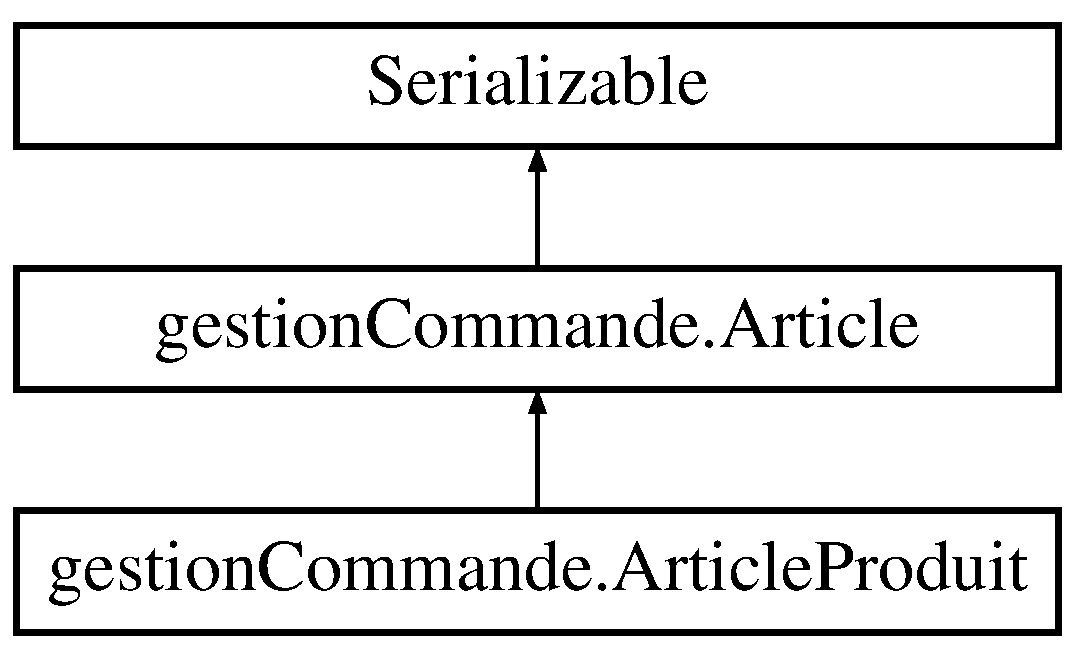
\includegraphics[height=3.000000cm]{classgestion_commande_1_1_article_produit}
\end{center}
\end{figure}
\subsection*{Public Member Functions}
\begin{DoxyCompactItemize}
\item 
float \hyperlink{classgestion_commande_1_1_article_produit_a9841bb3b200eebed8f41d693be10cffe}{get\-Cout\-Fabrication} ()
\begin{DoxyCompactList}\small\item\em Methode recuperant le cout de fabrication de l'article. \end{DoxyCompactList}\item 
void \hyperlink{classgestion_commande_1_1_article_produit_a4f8d0da086aa398f89f67384b3933de7}{saisir\-Article} ()
\begin{DoxyCompactList}\small\item\em Methode permettant la saisie d'un nouvel article. \end{DoxyCompactList}\item 
void \hyperlink{classgestion_commande_1_1_article_produit_aa6c49e11ed8fddd9088d98afb481e9d8}{afficher\-Article} ()
\begin{DoxyCompactList}\small\item\em Methode permettant d'afficher les informations de l'article. \end{DoxyCompactList}\end{DoxyCompactItemize}


\subsection{Detailed Description}
La classe \hyperlink{classgestion_commande_1_1_article_produit}{Article\-Produit} sert a instancier de nouveaux articles, ces articles sont ceux fabriques par l'entreprise. Les articles sont renseignes par leur nom, leur prix a l'unite et leur quantite en stock en plus du cout de fabrication. La classe \hyperlink{classgestion_commande_1_1_article_produit}{Article\-Produit} herite de la classe \hyperlink{classgestion_commande_1_1_article}{Article}. \begin{DoxyAuthor}{Author}
Rouinsard 
\end{DoxyAuthor}


Definition at line 8 of file Article\-Produit.\-java.



\subsection{Member Function Documentation}
\hypertarget{classgestion_commande_1_1_article_produit_aa6c49e11ed8fddd9088d98afb481e9d8}{\index{gestion\-Commande\-::\-Article\-Produit@{gestion\-Commande\-::\-Article\-Produit}!afficher\-Article@{afficher\-Article}}
\index{afficher\-Article@{afficher\-Article}!gestionCommande::ArticleProduit@{gestion\-Commande\-::\-Article\-Produit}}
\subsubsection[{afficher\-Article}]{\setlength{\rightskip}{0pt plus 5cm}void gestion\-Commande.\-Article\-Produit.\-afficher\-Article (
\begin{DoxyParamCaption}
{}
\end{DoxyParamCaption}
)}}\label{classgestion_commande_1_1_article_produit_aa6c49e11ed8fddd9088d98afb481e9d8}


Methode permettant d'afficher les informations de l'article. 

On utilise un super.\-afficher\-Article de la classe \hyperlink{classgestion_commande_1_1_article}{Article}. 

Definition at line 31 of file Article\-Produit.\-java.

\hypertarget{classgestion_commande_1_1_article_produit_a9841bb3b200eebed8f41d693be10cffe}{\index{gestion\-Commande\-::\-Article\-Produit@{gestion\-Commande\-::\-Article\-Produit}!get\-Cout\-Fabrication@{get\-Cout\-Fabrication}}
\index{get\-Cout\-Fabrication@{get\-Cout\-Fabrication}!gestionCommande::ArticleProduit@{gestion\-Commande\-::\-Article\-Produit}}
\subsubsection[{get\-Cout\-Fabrication}]{\setlength{\rightskip}{0pt plus 5cm}float gestion\-Commande.\-Article\-Produit.\-get\-Cout\-Fabrication (
\begin{DoxyParamCaption}
{}
\end{DoxyParamCaption}
)}}\label{classgestion_commande_1_1_article_produit_a9841bb3b200eebed8f41d693be10cffe}


Methode recuperant le cout de fabrication de l'article. 

\begin{DoxyReturn}{Returns}
this.\-cout\-Fabrication Correspond au cout de fabrication de l'article. 
\end{DoxyReturn}


Definition at line 14 of file Article\-Produit.\-java.

\hypertarget{classgestion_commande_1_1_article_produit_a4f8d0da086aa398f89f67384b3933de7}{\index{gestion\-Commande\-::\-Article\-Produit@{gestion\-Commande\-::\-Article\-Produit}!saisir\-Article@{saisir\-Article}}
\index{saisir\-Article@{saisir\-Article}!gestionCommande::ArticleProduit@{gestion\-Commande\-::\-Article\-Produit}}
\subsubsection[{saisir\-Article}]{\setlength{\rightskip}{0pt plus 5cm}void gestion\-Commande.\-Article\-Produit.\-saisir\-Article (
\begin{DoxyParamCaption}
{}
\end{DoxyParamCaption}
)}}\label{classgestion_commande_1_1_article_produit_a4f8d0da086aa398f89f67384b3933de7}


Methode permettant la saisie d'un nouvel article. 

Cette methode utilise la classe \hyperlink{classgestion_commande_1_1_lire}{Lire}.

La saisie d'un nouvel article se fait a partir d'un super permettant d'acceder a la methode saisir\-Article de la classe \hyperlink{classgestion_commande_1_1_article}{Article} auquel on ajoute un cout de fabrication. 

Definition at line 22 of file Article\-Produit.\-java.



The documentation for this class was generated from the following file\-:\begin{DoxyCompactItemize}
\item 
C\-:/\-Users/\-Rouinsard/\-Java/\-Gestion de commandes/src/gestion\-Commande/\hyperlink{_article_produit_8java}{Article\-Produit.\-java}\end{DoxyCompactItemize}

\hypertarget{classgestion_commande_1_1_client}{\section{gestion\-Commande.\-Client Class Reference}
\label{classgestion_commande_1_1_client}\index{gestion\-Commande.\-Client@{gestion\-Commande.\-Client}}
}
Inheritance diagram for gestion\-Commande.\-Client\-:\begin{figure}[H]
\begin{center}
\leavevmode
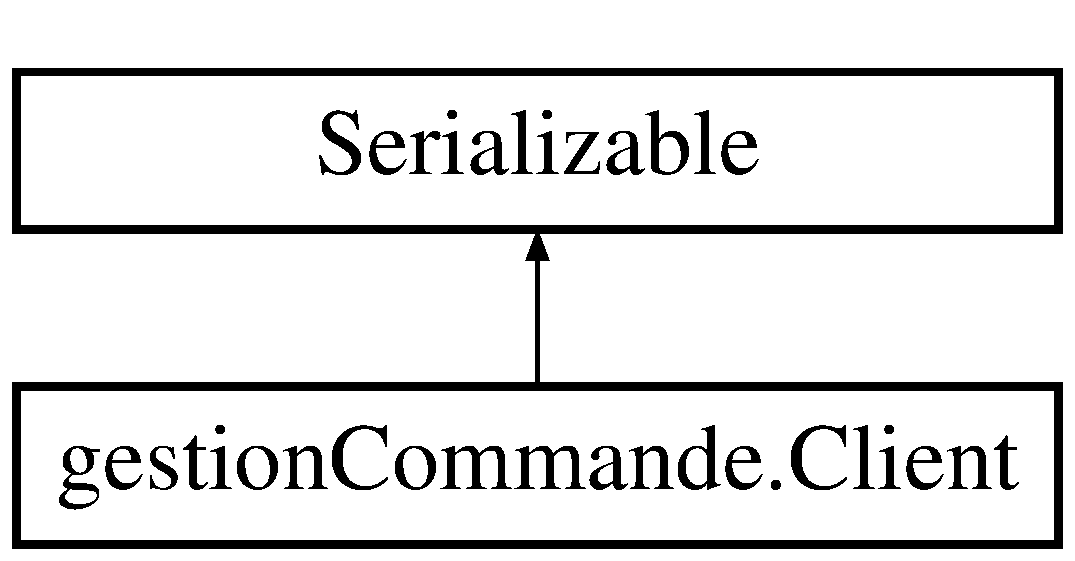
\includegraphics[height=2.000000cm]{classgestion_commande_1_1_client}
\end{center}
\end{figure}
\subsection*{Public Member Functions}
\begin{DoxyCompactItemize}
\item 
void \hyperlink{classgestion_commande_1_1_client_a4321a476e46367fb05288dd404681d18}{saisir\-Client} ()
\begin{DoxyCompactList}\small\item\em Methode permettant la saisie du client par l'utilisateur. \end{DoxyCompactList}\item 
void \hyperlink{classgestion_commande_1_1_client_a53a0a0f32d6749b1e024d25358df95c2}{afficher\-Client} ()
\begin{DoxyCompactList}\small\item\em Methode permettant l'affichage du client. \end{DoxyCompactList}\item 
void \hyperlink{classgestion_commande_1_1_client_aae19e5e1047008ebc311a60f8bba12ef}{saisir\-Adresse} ()
\begin{DoxyCompactList}\small\item\em Methode permettant de saisir uniquement l'adresse du client. \end{DoxyCompactList}\item 
void \hyperlink{classgestion_commande_1_1_client_a43705de1f5aabccba0b82e608eb7be36}{saisir\-Mail} ()
\begin{DoxyCompactList}\small\item\em Methode permettant de saisir uniquement l'adresse e-\/mail du client. \end{DoxyCompactList}\item 
void \hyperlink{classgestion_commande_1_1_client_ad05b1382806adbf2dbbe3ba3ae87873c}{saisir\-Tel} ()
\begin{DoxyCompactList}\small\item\em Methode permettant de saisir uniquement le numero de telephone du client. \end{DoxyCompactList}\item 
void \hyperlink{classgestion_commande_1_1_client_a69d2d1c75ffe66dd5eec68eecacbe2ec}{saisir\-Fax} ()
\begin{DoxyCompactList}\small\item\em Methode permettant de saisir uniquement le numero de fax du client. \end{DoxyCompactList}\item 
String \hyperlink{classgestion_commande_1_1_client_a571b28e84f725329bb1f1d3eaee45559}{get\-Nom} ()
\begin{DoxyCompactList}\small\item\em Methode permettant de recuperer le nom du client. \end{DoxyCompactList}\item 
String \hyperlink{classgestion_commande_1_1_client_a3d39bb4646c3127d1e1442a1d5d509b7}{get\-Adresse} ()
\begin{DoxyCompactList}\small\item\em Methode permettant de recuperer l'adresse du client. \end{DoxyCompactList}\item 
String \hyperlink{classgestion_commande_1_1_client_aada1d9e19fbd79dd328aa974d1fb6a32}{get\-Mail} ()
\begin{DoxyCompactList}\small\item\em Methode permettant de recuperer l'adresse e-\/mail du client. \end{DoxyCompactList}\item 
String \hyperlink{classgestion_commande_1_1_client_ade639183bc4dcf084cdaa0b2cb5f7f78}{get\-Tel} ()
\begin{DoxyCompactList}\small\item\em Methode permettant de recuperer le numero de telephone du client. \end{DoxyCompactList}\item 
String \hyperlink{classgestion_commande_1_1_client_a63fd3f7825b06ebc2f80c281801da179}{get\-Fax} ()
\begin{DoxyCompactList}\small\item\em Methode permettant de recuperer le numero de fax du client. \end{DoxyCompactList}\end{DoxyCompactItemize}
\subsection*{Static Public Member Functions}
\begin{DoxyCompactItemize}
\item 
static \hyperlink{classgestion_commande_1_1_client}{Client} \hyperlink{classgestion_commande_1_1_client_a3c011b7f3d17b2dc4b391533ff9a28ce}{recherche\-Client} (String un\-Nom, Array\-List$<$ \hyperlink{classgestion_commande_1_1_client}{Client} $>$ un\-Tab\-Client)
\begin{DoxyCompactList}\small\item\em Methode permettant de rechercher un client dans une collection. \end{DoxyCompactList}\end{DoxyCompactItemize}


\subsection{Detailed Description}
La classe \hyperlink{classgestion_commande_1_1_client}{Client} sert a instancier de nouveaux clients. Les clients sont renseignes par leur nom et leur adresse. La classe \hyperlink{classgestion_commande_1_1_client}{Client} implemente l'interface Serializable. \begin{DoxyAuthor}{Author}
Rouinsard 
\end{DoxyAuthor}


Definition at line 10 of file Client.\-java.



\subsection{Member Function Documentation}
\hypertarget{classgestion_commande_1_1_client_a53a0a0f32d6749b1e024d25358df95c2}{\index{gestion\-Commande\-::\-Client@{gestion\-Commande\-::\-Client}!afficher\-Client@{afficher\-Client}}
\index{afficher\-Client@{afficher\-Client}!gestionCommande::Client@{gestion\-Commande\-::\-Client}}
\subsubsection[{afficher\-Client}]{\setlength{\rightskip}{0pt plus 5cm}void gestion\-Commande.\-Client.\-afficher\-Client (
\begin{DoxyParamCaption}
{}
\end{DoxyParamCaption}
)}}\label{classgestion_commande_1_1_client_a53a0a0f32d6749b1e024d25358df95c2}


Methode permettant l'affichage du client. 



Definition at line 36 of file Client.\-java.

\hypertarget{classgestion_commande_1_1_client_a3d39bb4646c3127d1e1442a1d5d509b7}{\index{gestion\-Commande\-::\-Client@{gestion\-Commande\-::\-Client}!get\-Adresse@{get\-Adresse}}
\index{get\-Adresse@{get\-Adresse}!gestionCommande::Client@{gestion\-Commande\-::\-Client}}
\subsubsection[{get\-Adresse}]{\setlength{\rightskip}{0pt plus 5cm}String gestion\-Commande.\-Client.\-get\-Adresse (
\begin{DoxyParamCaption}
{}
\end{DoxyParamCaption}
)}}\label{classgestion_commande_1_1_client_a3d39bb4646c3127d1e1442a1d5d509b7}


Methode permettant de recuperer l'adresse du client. 

\begin{DoxyReturn}{Returns}
this.\-adr\-Client Correspond a l'adresse du client. 
\end{DoxyReturn}


Definition at line 80 of file Client.\-java.

\hypertarget{classgestion_commande_1_1_client_a63fd3f7825b06ebc2f80c281801da179}{\index{gestion\-Commande\-::\-Client@{gestion\-Commande\-::\-Client}!get\-Fax@{get\-Fax}}
\index{get\-Fax@{get\-Fax}!gestionCommande::Client@{gestion\-Commande\-::\-Client}}
\subsubsection[{get\-Fax}]{\setlength{\rightskip}{0pt plus 5cm}String gestion\-Commande.\-Client.\-get\-Fax (
\begin{DoxyParamCaption}
{}
\end{DoxyParamCaption}
)}}\label{classgestion_commande_1_1_client_a63fd3f7825b06ebc2f80c281801da179}


Methode permettant de recuperer le numero de fax du client. 

\begin{DoxyReturn}{Returns}
this.\-fax\-Client Correspond au numero de fax du client. 
\end{DoxyReturn}


Definition at line 101 of file Client.\-java.

\hypertarget{classgestion_commande_1_1_client_aada1d9e19fbd79dd328aa974d1fb6a32}{\index{gestion\-Commande\-::\-Client@{gestion\-Commande\-::\-Client}!get\-Mail@{get\-Mail}}
\index{get\-Mail@{get\-Mail}!gestionCommande::Client@{gestion\-Commande\-::\-Client}}
\subsubsection[{get\-Mail}]{\setlength{\rightskip}{0pt plus 5cm}String gestion\-Commande.\-Client.\-get\-Mail (
\begin{DoxyParamCaption}
{}
\end{DoxyParamCaption}
)}}\label{classgestion_commande_1_1_client_aada1d9e19fbd79dd328aa974d1fb6a32}


Methode permettant de recuperer l'adresse e-\/mail du client. 

\begin{DoxyReturn}{Returns}
this.\-adr\-Email Correspond a l'adresse e-\/mail du client. 
\end{DoxyReturn}


Definition at line 87 of file Client.\-java.

\hypertarget{classgestion_commande_1_1_client_a571b28e84f725329bb1f1d3eaee45559}{\index{gestion\-Commande\-::\-Client@{gestion\-Commande\-::\-Client}!get\-Nom@{get\-Nom}}
\index{get\-Nom@{get\-Nom}!gestionCommande::Client@{gestion\-Commande\-::\-Client}}
\subsubsection[{get\-Nom}]{\setlength{\rightskip}{0pt plus 5cm}String gestion\-Commande.\-Client.\-get\-Nom (
\begin{DoxyParamCaption}
{}
\end{DoxyParamCaption}
)}}\label{classgestion_commande_1_1_client_a571b28e84f725329bb1f1d3eaee45559}


Methode permettant de recuperer le nom du client. 

\begin{DoxyReturn}{Returns}
this.\-nom\-Client Correspond au nom du client. 
\end{DoxyReturn}


Definition at line 73 of file Client.\-java.

\hypertarget{classgestion_commande_1_1_client_ade639183bc4dcf084cdaa0b2cb5f7f78}{\index{gestion\-Commande\-::\-Client@{gestion\-Commande\-::\-Client}!get\-Tel@{get\-Tel}}
\index{get\-Tel@{get\-Tel}!gestionCommande::Client@{gestion\-Commande\-::\-Client}}
\subsubsection[{get\-Tel}]{\setlength{\rightskip}{0pt plus 5cm}String gestion\-Commande.\-Client.\-get\-Tel (
\begin{DoxyParamCaption}
{}
\end{DoxyParamCaption}
)}}\label{classgestion_commande_1_1_client_ade639183bc4dcf084cdaa0b2cb5f7f78}


Methode permettant de recuperer le numero de telephone du client. 

\begin{DoxyReturn}{Returns}
this.\-tel\-Client Correspond au numero de telephone du client. 
\end{DoxyReturn}


Definition at line 94 of file Client.\-java.

\hypertarget{classgestion_commande_1_1_client_a3c011b7f3d17b2dc4b391533ff9a28ce}{\index{gestion\-Commande\-::\-Client@{gestion\-Commande\-::\-Client}!recherche\-Client@{recherche\-Client}}
\index{recherche\-Client@{recherche\-Client}!gestionCommande::Client@{gestion\-Commande\-::\-Client}}
\subsubsection[{recherche\-Client}]{\setlength{\rightskip}{0pt plus 5cm}static {\bf Client} gestion\-Commande.\-Client.\-recherche\-Client (
\begin{DoxyParamCaption}
\item[{String}]{un\-Nom, }
\item[{Array\-List$<$ {\bf Client} $>$}]{un\-Tab\-Client}
\end{DoxyParamCaption}
)\hspace{0.3cm}{\ttfamily [static]}}}\label{classgestion_commande_1_1_client_a3c011b7f3d17b2dc4b391533ff9a28ce}


Methode permettant de rechercher un client dans une collection. 

Cette methode recherche un client a partir de son nom dans une collection passee en parametre, puis la fonction renvoie un client ou null si aucun client n'a pu etre trouvee. 
\begin{DoxyParams}{Parameters}
{\em un\-Nom} & Correspond au nom du client que l'on recherche. \\
\hline
{\em un\-Tab\-Client} & Correspond a la collection dans laquelle on recherche le client. \\
\hline
\end{DoxyParams}
\begin{DoxyReturn}{Returns}
\hyperlink{classgestion_commande_1_1_client}{Client} 
\end{DoxyReturn}


Definition at line 111 of file Client.\-java.

\hypertarget{classgestion_commande_1_1_client_aae19e5e1047008ebc311a60f8bba12ef}{\index{gestion\-Commande\-::\-Client@{gestion\-Commande\-::\-Client}!saisir\-Adresse@{saisir\-Adresse}}
\index{saisir\-Adresse@{saisir\-Adresse}!gestionCommande::Client@{gestion\-Commande\-::\-Client}}
\subsubsection[{saisir\-Adresse}]{\setlength{\rightskip}{0pt plus 5cm}void gestion\-Commande.\-Client.\-saisir\-Adresse (
\begin{DoxyParamCaption}
{}
\end{DoxyParamCaption}
)}}\label{classgestion_commande_1_1_client_aae19e5e1047008ebc311a60f8bba12ef}


Methode permettant de saisir uniquement l'adresse du client. 

Permet de saisir uniquement l'adresse du client afin de pouvoir modifier celle-\/ci sans alterer les autres attributs du client. Cette methode utilise egalement la classe \hyperlink{classgestion_commande_1_1_lire}{Lire}. 

Definition at line 44 of file Client.\-java.

\hypertarget{classgestion_commande_1_1_client_a4321a476e46367fb05288dd404681d18}{\index{gestion\-Commande\-::\-Client@{gestion\-Commande\-::\-Client}!saisir\-Client@{saisir\-Client}}
\index{saisir\-Client@{saisir\-Client}!gestionCommande::Client@{gestion\-Commande\-::\-Client}}
\subsubsection[{saisir\-Client}]{\setlength{\rightskip}{0pt plus 5cm}void gestion\-Commande.\-Client.\-saisir\-Client (
\begin{DoxyParamCaption}
{}
\end{DoxyParamCaption}
)}}\label{classgestion_commande_1_1_client_a4321a476e46367fb05288dd404681d18}


Methode permettant la saisie du client par l'utilisateur. 

La saisie utilise la classe \hyperlink{classgestion_commande_1_1_lire}{Lire}, afin que l'utilisateur puisse saisir les donnees. 

Definition at line 20 of file Client.\-java.

\hypertarget{classgestion_commande_1_1_client_a69d2d1c75ffe66dd5eec68eecacbe2ec}{\index{gestion\-Commande\-::\-Client@{gestion\-Commande\-::\-Client}!saisir\-Fax@{saisir\-Fax}}
\index{saisir\-Fax@{saisir\-Fax}!gestionCommande::Client@{gestion\-Commande\-::\-Client}}
\subsubsection[{saisir\-Fax}]{\setlength{\rightskip}{0pt plus 5cm}void gestion\-Commande.\-Client.\-saisir\-Fax (
\begin{DoxyParamCaption}
{}
\end{DoxyParamCaption}
)}}\label{classgestion_commande_1_1_client_a69d2d1c75ffe66dd5eec68eecacbe2ec}


Methode permettant de saisir uniquement le numero de fax du client. 



Definition at line 65 of file Client.\-java.

\hypertarget{classgestion_commande_1_1_client_a43705de1f5aabccba0b82e608eb7be36}{\index{gestion\-Commande\-::\-Client@{gestion\-Commande\-::\-Client}!saisir\-Mail@{saisir\-Mail}}
\index{saisir\-Mail@{saisir\-Mail}!gestionCommande::Client@{gestion\-Commande\-::\-Client}}
\subsubsection[{saisir\-Mail}]{\setlength{\rightskip}{0pt plus 5cm}void gestion\-Commande.\-Client.\-saisir\-Mail (
\begin{DoxyParamCaption}
{}
\end{DoxyParamCaption}
)}}\label{classgestion_commande_1_1_client_a43705de1f5aabccba0b82e608eb7be36}


Methode permettant de saisir uniquement l'adresse e-\/mail du client. 



Definition at line 51 of file Client.\-java.

\hypertarget{classgestion_commande_1_1_client_ad05b1382806adbf2dbbe3ba3ae87873c}{\index{gestion\-Commande\-::\-Client@{gestion\-Commande\-::\-Client}!saisir\-Tel@{saisir\-Tel}}
\index{saisir\-Tel@{saisir\-Tel}!gestionCommande::Client@{gestion\-Commande\-::\-Client}}
\subsubsection[{saisir\-Tel}]{\setlength{\rightskip}{0pt plus 5cm}void gestion\-Commande.\-Client.\-saisir\-Tel (
\begin{DoxyParamCaption}
{}
\end{DoxyParamCaption}
)}}\label{classgestion_commande_1_1_client_ad05b1382806adbf2dbbe3ba3ae87873c}


Methode permettant de saisir uniquement le numero de telephone du client. 



Definition at line 58 of file Client.\-java.



The documentation for this class was generated from the following file\-:\begin{DoxyCompactItemize}
\item 
C\-:/\-Users/\-Rouinsard/\-Java/\-Gestion de commandes/src/gestion\-Commande/\hyperlink{_client_8java}{Client.\-java}\end{DoxyCompactItemize}

\hypertarget{classgestion_commande_1_1_commande}{\section{gestion\-Commande.\-Commande Class Reference}
\label{classgestion_commande_1_1_commande}\index{gestion\-Commande.\-Commande@{gestion\-Commande.\-Commande}}
}
Inheritance diagram for gestion\-Commande.\-Commande\-:\begin{figure}[H]
\begin{center}
\leavevmode
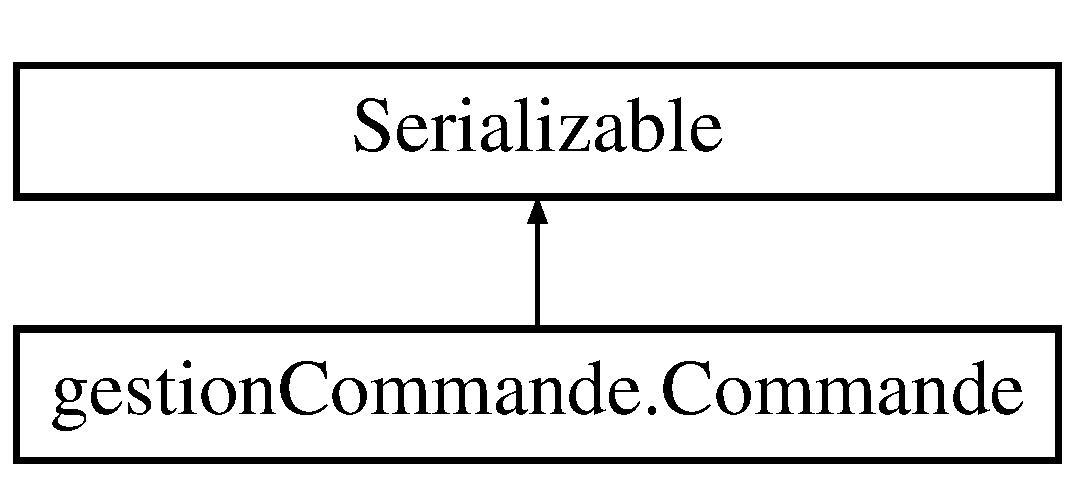
\includegraphics[height=2.000000cm]{classgestion_commande_1_1_commande}
\end{center}
\end{figure}
\subsection*{Public Member Functions}
\begin{DoxyCompactItemize}
\item 
\hyperlink{classgestion_commande_1_1_commande_a7e5dae85be4607d83b0cab36ba1dc463}{Commande} (long num, \hyperlink{classgestion_commande_1_1_client}{Client} cli, \hyperlink{classgestion_commande_1_1_article}{Article} art, int nb\-Commande)
\begin{DoxyCompactList}\small\item\em Constructeur de la classe commande. \end{DoxyCompactList}\item 
void \hyperlink{classgestion_commande_1_1_commande_a28e22a23c75689f346b8d130e3f326eb}{afficher\-Commande} ()
\begin{DoxyCompactList}\small\item\em Methode permettant d'afficher la commande. \end{DoxyCompactList}\item 
long \hyperlink{classgestion_commande_1_1_commande_a06ffc43c81c0593d268c919de63ed02c}{get\-Num} ()
\begin{DoxyCompactList}\small\item\em Methode permettant de recuperer le numero de commande. \end{DoxyCompactList}\item 
\hyperlink{classgestion_commande_1_1_client}{Client} \hyperlink{classgestion_commande_1_1_commande_aeaa08b1cafcdb48bcc6f70066a949f23}{get\-Client} ()
\begin{DoxyCompactList}\small\item\em Methode permettant de recuperer le client de la commande. \end{DoxyCompactList}\item 
\hyperlink{classgestion_commande_1_1_article}{Article} \hyperlink{classgestion_commande_1_1_commande_a5bc20e7184b4d85e5fbbcbbe05c5aa4e}{get\-Article} ()
\begin{DoxyCompactList}\small\item\em Methode permettant de recuperer l'article de la commande. \end{DoxyCompactList}\item 
int \hyperlink{classgestion_commande_1_1_commande_a11f2c59ee953a83bb7740655ca17dca2}{get\-Quantite\-Commande} ()
\begin{DoxyCompactList}\small\item\em Methode permettant de recuperer la quantite commandee. \end{DoxyCompactList}\end{DoxyCompactItemize}


\subsection{Detailed Description}
La classe \hyperlink{classgestion_commande_1_1_commande}{Commande} sert a instancier de nouvelles commandes. Les commandes sont renseignes par leur numero unique, leur client et l'article commandee par ce client. La classe \hyperlink{classgestion_commande_1_1_commande}{Commande} implemente l'interface Serializable. \begin{DoxyAuthor}{Author}
Rouinsard 
\end{DoxyAuthor}


Definition at line 11 of file Commande.\-java.



\subsection{Constructor \& Destructor Documentation}
\hypertarget{classgestion_commande_1_1_commande_a7e5dae85be4607d83b0cab36ba1dc463}{\index{gestion\-Commande\-::\-Commande@{gestion\-Commande\-::\-Commande}!Commande@{Commande}}
\index{Commande@{Commande}!gestionCommande::Commande@{gestion\-Commande\-::\-Commande}}
\subsubsection[{Commande}]{\setlength{\rightskip}{0pt plus 5cm}gestion\-Commande.\-Commande.\-Commande (
\begin{DoxyParamCaption}
\item[{long}]{num, }
\item[{{\bf Client}}]{cli, }
\item[{{\bf Article}}]{art, }
\item[{int}]{nb\-Commande}
\end{DoxyParamCaption}
)}}\label{classgestion_commande_1_1_commande_a7e5dae85be4607d83b0cab36ba1dc463}


Constructeur de la classe commande. 

Le constructeur de la classe commande prenant en parametre un numero d'id, un client et un article. 
\begin{DoxyParams}{Parameters}
{\em num} & Un numero de commande unique. \\
\hline
{\em cli} & Le client effectuant la commande. \\
\hline
{\em art} & L'article commandee par le client. \\
\hline
\end{DoxyParams}


Definition at line 23 of file Commande.\-java.



\subsection{Member Function Documentation}
\hypertarget{classgestion_commande_1_1_commande_a28e22a23c75689f346b8d130e3f326eb}{\index{gestion\-Commande\-::\-Commande@{gestion\-Commande\-::\-Commande}!afficher\-Commande@{afficher\-Commande}}
\index{afficher\-Commande@{afficher\-Commande}!gestionCommande::Commande@{gestion\-Commande\-::\-Commande}}
\subsubsection[{afficher\-Commande}]{\setlength{\rightskip}{0pt plus 5cm}void gestion\-Commande.\-Commande.\-afficher\-Commande (
\begin{DoxyParamCaption}
{}
\end{DoxyParamCaption}
)}}\label{classgestion_commande_1_1_commande_a28e22a23c75689f346b8d130e3f326eb}


Methode permettant d'afficher la commande. 

Cette methode affiche le numero unique de la commande, puis recupere le nom du client grace a la methode ge\-Nom() de la classe \hyperlink{classgestion_commande_1_1_client}{Client}, ainsi que le nom de l'article et le prix a l'unite de celui-\/ci via les methodes get\-Nom\-Article() et get\-Prix\-Uniraite() de la classe \hyperlink{classgestion_commande_1_1_article}{Article}. 

Definition at line 33 of file Commande.\-java.

\hypertarget{classgestion_commande_1_1_commande_a5bc20e7184b4d85e5fbbcbbe05c5aa4e}{\index{gestion\-Commande\-::\-Commande@{gestion\-Commande\-::\-Commande}!get\-Article@{get\-Article}}
\index{get\-Article@{get\-Article}!gestionCommande::Commande@{gestion\-Commande\-::\-Commande}}
\subsubsection[{get\-Article}]{\setlength{\rightskip}{0pt plus 5cm}{\bf Article} gestion\-Commande.\-Commande.\-get\-Article (
\begin{DoxyParamCaption}
{}
\end{DoxyParamCaption}
)}}\label{classgestion_commande_1_1_commande_a5bc20e7184b4d85e5fbbcbbe05c5aa4e}


Methode permettant de recuperer l'article de la commande. 

\begin{DoxyReturn}{Returns}
this.\-larticle Correspond a l'article de la commande. 
\end{DoxyReturn}


Definition at line 56 of file Commande.\-java.

\hypertarget{classgestion_commande_1_1_commande_aeaa08b1cafcdb48bcc6f70066a949f23}{\index{gestion\-Commande\-::\-Commande@{gestion\-Commande\-::\-Commande}!get\-Client@{get\-Client}}
\index{get\-Client@{get\-Client}!gestionCommande::Commande@{gestion\-Commande\-::\-Commande}}
\subsubsection[{get\-Client}]{\setlength{\rightskip}{0pt plus 5cm}{\bf Client} gestion\-Commande.\-Commande.\-get\-Client (
\begin{DoxyParamCaption}
{}
\end{DoxyParamCaption}
)}}\label{classgestion_commande_1_1_commande_aeaa08b1cafcdb48bcc6f70066a949f23}


Methode permettant de recuperer le client de la commande. 

\begin{DoxyReturn}{Returns}
this.\-le\-Client Correspond au client de la commande. 
\end{DoxyReturn}


Definition at line 49 of file Commande.\-java.

\hypertarget{classgestion_commande_1_1_commande_a06ffc43c81c0593d268c919de63ed02c}{\index{gestion\-Commande\-::\-Commande@{gestion\-Commande\-::\-Commande}!get\-Num@{get\-Num}}
\index{get\-Num@{get\-Num}!gestionCommande::Commande@{gestion\-Commande\-::\-Commande}}
\subsubsection[{get\-Num}]{\setlength{\rightskip}{0pt plus 5cm}long gestion\-Commande.\-Commande.\-get\-Num (
\begin{DoxyParamCaption}
{}
\end{DoxyParamCaption}
)}}\label{classgestion_commande_1_1_commande_a06ffc43c81c0593d268c919de63ed02c}


Methode permettant de recuperer le numero de commande. 

\begin{DoxyReturn}{Returns}
this.\-num\-Cde Correspond au numero de la commande. 
\end{DoxyReturn}


Definition at line 42 of file Commande.\-java.

\hypertarget{classgestion_commande_1_1_commande_a11f2c59ee953a83bb7740655ca17dca2}{\index{gestion\-Commande\-::\-Commande@{gestion\-Commande\-::\-Commande}!get\-Quantite\-Commande@{get\-Quantite\-Commande}}
\index{get\-Quantite\-Commande@{get\-Quantite\-Commande}!gestionCommande::Commande@{gestion\-Commande\-::\-Commande}}
\subsubsection[{get\-Quantite\-Commande}]{\setlength{\rightskip}{0pt plus 5cm}int gestion\-Commande.\-Commande.\-get\-Quantite\-Commande (
\begin{DoxyParamCaption}
{}
\end{DoxyParamCaption}
)}}\label{classgestion_commande_1_1_commande_a11f2c59ee953a83bb7740655ca17dca2}


Methode permettant de recuperer la quantite commandee. 

\begin{DoxyReturn}{Returns}
this.\-qte\-Commande Correspond a la quantite commandee. 
\end{DoxyReturn}


Definition at line 63 of file Commande.\-java.



The documentation for this class was generated from the following file\-:\begin{DoxyCompactItemize}
\item 
C\-:/\-Users/\-Rouinsard/\-Java/\-Gestion de commandes/src/gestion\-Commande/\hyperlink{_commande_8java}{Commande.\-java}\end{DoxyCompactItemize}

\hypertarget{classgestion_commande_1_1_lire}{\section{gestion\-Commande.\-Lire Class Reference}
\label{classgestion_commande_1_1_lire}\index{gestion\-Commande.\-Lire@{gestion\-Commande.\-Lire}}
}
\subsection*{Static Public Member Functions}
\begin{DoxyCompactItemize}
\item 
static String \hyperlink{classgestion_commande_1_1_lire_a80bc00afc8ee00cdf98d844099184e16}{S} ()
\item 
static byte \hyperlink{classgestion_commande_1_1_lire_a594d6557a659d35a7de8f140f090b38c}{b} ()
\item 
static short \hyperlink{classgestion_commande_1_1_lire_a5b17d4c1ebafa4c2f3248e25dc0abfb3}{s} ()
\item 
static int \hyperlink{classgestion_commande_1_1_lire_a4c849f256ceef5c7d7f025bf7870fea6}{i} ()
\item 
static long \hyperlink{classgestion_commande_1_1_lire_ae903197e030dcb46c1b527a3b4e69374}{l} ()
\item 
static double \hyperlink{classgestion_commande_1_1_lire_a4219a16fbeafd478ea01a9528c3bb5bd}{d} ()
\item 
static float \hyperlink{classgestion_commande_1_1_lire_a007ba2d3004f27d3040f409074aab7f8}{f} ()
\item 
static char \hyperlink{classgestion_commande_1_1_lire_a4b31da4cd5affa5a3c46768572aaccd6}{c} ()
\end{DoxyCompactItemize}


\subsection{Detailed Description}


Definition at line 4 of file Lire.\-java.



\subsection{Member Function Documentation}
\hypertarget{classgestion_commande_1_1_lire_a594d6557a659d35a7de8f140f090b38c}{\index{gestion\-Commande\-::\-Lire@{gestion\-Commande\-::\-Lire}!b@{b}}
\index{b@{b}!gestionCommande::Lire@{gestion\-Commande\-::\-Lire}}
\subsubsection[{b}]{\setlength{\rightskip}{0pt plus 5cm}static byte gestion\-Commande.\-Lire.\-b (
\begin{DoxyParamCaption}
{}
\end{DoxyParamCaption}
)\hspace{0.3cm}{\ttfamily [static]}}}\label{classgestion_commande_1_1_lire_a594d6557a659d35a7de8f140f090b38c}


Definition at line 25 of file Lire.\-java.

\hypertarget{classgestion_commande_1_1_lire_a4b31da4cd5affa5a3c46768572aaccd6}{\index{gestion\-Commande\-::\-Lire@{gestion\-Commande\-::\-Lire}!c@{c}}
\index{c@{c}!gestionCommande::Lire@{gestion\-Commande\-::\-Lire}}
\subsubsection[{c}]{\setlength{\rightskip}{0pt plus 5cm}static char gestion\-Commande.\-Lire.\-c (
\begin{DoxyParamCaption}
{}
\end{DoxyParamCaption}
)\hspace{0.3cm}{\ttfamily [static]}}}\label{classgestion_commande_1_1_lire_a4b31da4cd5affa5a3c46768572aaccd6}


Definition at line 104 of file Lire.\-java.

\hypertarget{classgestion_commande_1_1_lire_a4219a16fbeafd478ea01a9528c3bb5bd}{\index{gestion\-Commande\-::\-Lire@{gestion\-Commande\-::\-Lire}!d@{d}}
\index{d@{d}!gestionCommande::Lire@{gestion\-Commande\-::\-Lire}}
\subsubsection[{d}]{\setlength{\rightskip}{0pt plus 5cm}static double gestion\-Commande.\-Lire.\-d (
\begin{DoxyParamCaption}
{}
\end{DoxyParamCaption}
)\hspace{0.3cm}{\ttfamily [static]}}}\label{classgestion_commande_1_1_lire_a4219a16fbeafd478ea01a9528c3bb5bd}


Definition at line 77 of file Lire.\-java.

\hypertarget{classgestion_commande_1_1_lire_a007ba2d3004f27d3040f409074aab7f8}{\index{gestion\-Commande\-::\-Lire@{gestion\-Commande\-::\-Lire}!f@{f}}
\index{f@{f}!gestionCommande::Lire@{gestion\-Commande\-::\-Lire}}
\subsubsection[{f}]{\setlength{\rightskip}{0pt plus 5cm}static float gestion\-Commande.\-Lire.\-f (
\begin{DoxyParamCaption}
{}
\end{DoxyParamCaption}
)\hspace{0.3cm}{\ttfamily [static]}}}\label{classgestion_commande_1_1_lire_a007ba2d3004f27d3040f409074aab7f8}


Definition at line 90 of file Lire.\-java.

\hypertarget{classgestion_commande_1_1_lire_a4c849f256ceef5c7d7f025bf7870fea6}{\index{gestion\-Commande\-::\-Lire@{gestion\-Commande\-::\-Lire}!i@{i}}
\index{i@{i}!gestionCommande::Lire@{gestion\-Commande\-::\-Lire}}
\subsubsection[{i}]{\setlength{\rightskip}{0pt plus 5cm}static int gestion\-Commande.\-Lire.\-i (
\begin{DoxyParamCaption}
{}
\end{DoxyParamCaption}
)\hspace{0.3cm}{\ttfamily [static]}}}\label{classgestion_commande_1_1_lire_a4c849f256ceef5c7d7f025bf7870fea6}


Definition at line 51 of file Lire.\-java.

\hypertarget{classgestion_commande_1_1_lire_ae903197e030dcb46c1b527a3b4e69374}{\index{gestion\-Commande\-::\-Lire@{gestion\-Commande\-::\-Lire}!l@{l}}
\index{l@{l}!gestionCommande::Lire@{gestion\-Commande\-::\-Lire}}
\subsubsection[{l}]{\setlength{\rightskip}{0pt plus 5cm}static long gestion\-Commande.\-Lire.\-l (
\begin{DoxyParamCaption}
{}
\end{DoxyParamCaption}
)\hspace{0.3cm}{\ttfamily [static]}}}\label{classgestion_commande_1_1_lire_ae903197e030dcb46c1b527a3b4e69374}


Definition at line 64 of file Lire.\-java.

\hypertarget{classgestion_commande_1_1_lire_a80bc00afc8ee00cdf98d844099184e16}{\index{gestion\-Commande\-::\-Lire@{gestion\-Commande\-::\-Lire}!S@{S}}
\index{S@{S}!gestionCommande::Lire@{gestion\-Commande\-::\-Lire}}
\subsubsection[{S}]{\setlength{\rightskip}{0pt plus 5cm}static String gestion\-Commande.\-Lire.\-S (
\begin{DoxyParamCaption}
{}
\end{DoxyParamCaption}
)\hspace{0.3cm}{\ttfamily [static]}}}\label{classgestion_commande_1_1_lire_a80bc00afc8ee00cdf98d844099184e16}


Definition at line 6 of file Lire.\-java.

\hypertarget{classgestion_commande_1_1_lire_a5b17d4c1ebafa4c2f3248e25dc0abfb3}{\index{gestion\-Commande\-::\-Lire@{gestion\-Commande\-::\-Lire}!s@{s}}
\index{s@{s}!gestionCommande::Lire@{gestion\-Commande\-::\-Lire}}
\subsubsection[{s}]{\setlength{\rightskip}{0pt plus 5cm}static short gestion\-Commande.\-Lire.\-s (
\begin{DoxyParamCaption}
{}
\end{DoxyParamCaption}
)\hspace{0.3cm}{\ttfamily [static]}}}\label{classgestion_commande_1_1_lire_a5b17d4c1ebafa4c2f3248e25dc0abfb3}


Definition at line 38 of file Lire.\-java.



The documentation for this class was generated from the following file\-:\begin{DoxyCompactItemize}
\item 
C\-:/\-Users/\-Rouinsard/\-Java/\-Gestion de commandes/src/gestion\-Commande/\hyperlink{_lire_8java}{Lire.\-java}\end{DoxyCompactItemize}

\hypertarget{classgestion_commande_1_1main}{\section{gestion\-Commande.\-main Class Reference}
\label{classgestion_commande_1_1main}\index{gestion\-Commande.\-main@{gestion\-Commande.\-main}}
}
\subsection*{Static Public Member Functions}
\begin{DoxyCompactItemize}
\item 
static void \hyperlink{classgestion_commande_1_1main_a0e5d4f61c1ddeb1175043ce260b5ee7e}{main} (String\mbox{[}$\,$\mbox{]} args)
\end{DoxyCompactItemize}


\subsection{Detailed Description}


Definition at line 12 of file main.\-java.



\subsection{Constructor \& Destructor Documentation}
\hypertarget{classgestion_commande_1_1main_a0e5d4f61c1ddeb1175043ce260b5ee7e}{\index{gestion\-Commande\-::main@{gestion\-Commande\-::main}!main@{main}}
\index{main@{main}!gestionCommande::main@{gestion\-Commande\-::main}}
\subsubsection[{main}]{\setlength{\rightskip}{0pt plus 5cm}static void gestion\-Commande.\-main.\-main (
\begin{DoxyParamCaption}
\item[{String\mbox{[}$\,$\mbox{]}}]{args}
\end{DoxyParamCaption}
)\hspace{0.3cm}{\ttfamily [static]}}}\label{classgestion_commande_1_1main_a0e5d4f61c1ddeb1175043ce260b5ee7e}


Definition at line 14 of file main.\-java.



The documentation for this class was generated from the following file\-:\begin{DoxyCompactItemize}
\item 
C\-:/\-Users/\-Rouinsard/\-Java/\-Gestion de commandes/src/gestion\-Commande/\hyperlink{main_8java}{main.\-java}\end{DoxyCompactItemize}

\chapter{File Documentation}
\hypertarget{_article_8java}{\section{C\-:/\-Users/\-Rouinsard/\-Java/\-Gestion de commandes/src/gestion\-Commande/\-Article.java File Reference}
\label{_article_8java}\index{C\-:/\-Users/\-Rouinsard/\-Java/\-Gestion de commandes/src/gestion\-Commande/\-Article.\-java@{C\-:/\-Users/\-Rouinsard/\-Java/\-Gestion de commandes/src/gestion\-Commande/\-Article.\-java}}
}
\subsection*{Classes}
\begin{DoxyCompactItemize}
\item 
class \hyperlink{classgestion_commande_1_1_article}{gestion\-Commande.\-Article}
\end{DoxyCompactItemize}
\subsection*{Packages}
\begin{DoxyCompactItemize}
\item 
package \hyperlink{namespacegestion_commande}{gestion\-Commande}
\end{DoxyCompactItemize}

\hypertarget{_article_produit_8java}{\section{C\-:/\-Users/\-Rouinsard/\-Java/\-Gestion de commandes/src/gestion\-Commande/\-Article\-Produit.java File Reference}
\label{_article_produit_8java}\index{C\-:/\-Users/\-Rouinsard/\-Java/\-Gestion de commandes/src/gestion\-Commande/\-Article\-Produit.\-java@{C\-:/\-Users/\-Rouinsard/\-Java/\-Gestion de commandes/src/gestion\-Commande/\-Article\-Produit.\-java}}
}
\subsection*{Classes}
\begin{DoxyCompactItemize}
\item 
class \hyperlink{classgestion_commande_1_1_article_produit}{gestion\-Commande.\-Article\-Produit}
\end{DoxyCompactItemize}
\subsection*{Packages}
\begin{DoxyCompactItemize}
\item 
package \hyperlink{namespacegestion_commande}{gestion\-Commande}
\end{DoxyCompactItemize}

\hypertarget{_client_8java}{\section{C\-:/\-Users/\-Rouinsard/\-Java/\-Gestion de commandes/src/gestion\-Commande/\-Client.java File Reference}
\label{_client_8java}\index{C\-:/\-Users/\-Rouinsard/\-Java/\-Gestion de commandes/src/gestion\-Commande/\-Client.\-java@{C\-:/\-Users/\-Rouinsard/\-Java/\-Gestion de commandes/src/gestion\-Commande/\-Client.\-java}}
}
\subsection*{Classes}
\begin{DoxyCompactItemize}
\item 
class \hyperlink{classgestion_commande_1_1_client}{gestion\-Commande.\-Client}
\end{DoxyCompactItemize}
\subsection*{Packages}
\begin{DoxyCompactItemize}
\item 
package \hyperlink{namespacegestion_commande}{gestion\-Commande}
\end{DoxyCompactItemize}

\hypertarget{_commande_8java}{\section{C\-:/\-Users/\-Rouinsard/\-Java/\-Gestion de commandes/src/gestion\-Commande/\-Commande.java File Reference}
\label{_commande_8java}\index{C\-:/\-Users/\-Rouinsard/\-Java/\-Gestion de commandes/src/gestion\-Commande/\-Commande.\-java@{C\-:/\-Users/\-Rouinsard/\-Java/\-Gestion de commandes/src/gestion\-Commande/\-Commande.\-java}}
}
\subsection*{Classes}
\begin{DoxyCompactItemize}
\item 
class \hyperlink{classgestion_commande_1_1_commande}{gestion\-Commande.\-Commande}
\end{DoxyCompactItemize}
\subsection*{Packages}
\begin{DoxyCompactItemize}
\item 
package \hyperlink{namespacegestion_commande}{gestion\-Commande}
\end{DoxyCompactItemize}

\hypertarget{_lire_8java}{\section{C\-:/\-Users/\-Rouinsard/\-Java/\-Gestion de commandes/src/gestion\-Commande/\-Lire.java File Reference}
\label{_lire_8java}\index{C\-:/\-Users/\-Rouinsard/\-Java/\-Gestion de commandes/src/gestion\-Commande/\-Lire.\-java@{C\-:/\-Users/\-Rouinsard/\-Java/\-Gestion de commandes/src/gestion\-Commande/\-Lire.\-java}}
}
\subsection*{Classes}
\begin{DoxyCompactItemize}
\item 
class \hyperlink{classgestion_commande_1_1_lire}{gestion\-Commande.\-Lire}
\end{DoxyCompactItemize}
\subsection*{Packages}
\begin{DoxyCompactItemize}
\item 
package \hyperlink{namespacegestion_commande}{gestion\-Commande}
\end{DoxyCompactItemize}

\hypertarget{main_8java}{\section{C\-:/\-Users/\-Rouinsard/\-Java/\-Gestion de commandes/src/gestion\-Commande/main.java File Reference}
\label{main_8java}\index{C\-:/\-Users/\-Rouinsard/\-Java/\-Gestion de commandes/src/gestion\-Commande/main.\-java@{C\-:/\-Users/\-Rouinsard/\-Java/\-Gestion de commandes/src/gestion\-Commande/main.\-java}}
}
\subsection*{Classes}
\begin{DoxyCompactItemize}
\item 
class \hyperlink{classgestion_commande_1_1main}{gestion\-Commande.\-main}
\end{DoxyCompactItemize}
\subsection*{Packages}
\begin{DoxyCompactItemize}
\item 
package \hyperlink{namespacegestion_commande}{gestion\-Commande}
\end{DoxyCompactItemize}

\addcontentsline{toc}{part}{Index}
\printindex
\end{document}
